\documentclass{article}
\usepackage[utf8]{inputenc}
\usepackage{array}
\usepackage{classeRapport}
\usepackage{enumitem}
\usepackage{times}
\usepackage{fancyhdr,graphicx,amsmath,amssymb, xcolor}
\usepackage[ruled,vlined, french]{algorithm2e}
    \SetKwInput{Declaration}{Declaration}
    \SetKw{KwA}{a}
    \SetKw{Retour}{retourner}
    \SetKwBlock{Deb}{debut}{fin}
    \SetKwIF{Si}{SinonSi}{Sinon}{si}{alors}{sinon si}{sinon}{finsi}
    \SetKwFor{Tq}{tant que}{faire}{finTantQue}
    \SetKwFor{Pour}{pour}{faire}{finPour}
    \SetKwRepeat{Repeter}{repeter}{jusqu’a}
    \SetKw{Pre}{Precondition(s)}

\usepackage{listings}
    \definecolor{darkWhite}{rgb}{0.94,0.94,0.94}
 
    \lstset{
      aboveskip=3mm,
      belowskip=-2mm,
      backgroundcolor=\color{darkWhite},
      basicstyle=\footnotesize,
      breakatwhitespace=false,
      breaklines=true,
      captionpos=b,
      commentstyle=\color{red},
      deletekeywords={...},
      escapeinside={\%*}{*)},
      extendedchars=true,
      framexleftmargin=16pt,
      framextopmargin=3pt,
      framexbottommargin=6pt,
      frame=tb,
      keepspaces=true,
      keywordstyle=\color{blue},
      language=C,
      literate=
      {²}{{\textsuperscript{2}}}1
      {⁴}{{\textsuperscript{4}}}1
      {⁶}{{\textsuperscript{6}}}1
      {⁸}{{\textsuperscript{8}}}1
      {€}{{\euro{}}}1
      {é}{{\'e}}1
      {è}{{\`{e}}}1
      {ê}{{\^{e}}}1
      {ë}{{\¨{e}}}1
      {É}{{\'{E}}}1
      {Ê}{{\^{E}}}1
      {û}{{\^{u}}}1
      {ù}{{\`{u}}}1
      {â}{{\^{a}}}1
      {à}{{\`{a}}}1
      {á}{{\'{a}}}1
      {ã}{{\~{a}}}1
      {Á}{{\'{A}}}1
      {Â}{{\^{A}}}1
      {Ã}{{\~{A}}}1
      {ç}{{\c{c}}}1
      {Ç}{{\c{C}}}1
      {õ}{{\~{o}}}1
      {ó}{{\'{o}}}1
      {ô}{{\^{o}}}1
      {Õ}{{\~{O}}}1
      {Ó}{{\'{O}}}1
      {Ô}{{\^{O}}}1
      {î}{{\^{i}}}1
      {Î}{{\^{I}}}1
      {í}{{\'{i}}}1
      {Í}{{\~{Í}}}1,
      morekeywords={*,...},
      numbers=left,
      numbersep=10pt,
      numberstyle=\tiny\color{black},
      rulecolor=\color{black},
      showspaces=false,
      showstringspaces=false,
      showtabs=false,
      stepnumber=1,
      stringstyle=\color{gray},
      tabsize=4,
      title=\lstname,
    }
\begin{document}

\PageDeGarde
{cover.png} % image sur la page de garde
{Compresseur de Huffman} % titre principal
{Depuis j'ai plus winrar} % sous-titre
{Julie \textsc{Allais}\\
Yassine \textsc{Ben Abderrahmane}\\
Antoine \textsc{Camusat}\\
Florine \textsc{Chevrier}\\
Florin \textsc{Croitoru}\\
Marine \textsc{Varlet}} % nom
{Algo – ITI3 – 2020} % bas de page


\Page{INSALogo} % logo de bas de page (en bas a droite)

\tableofcontents

\clearpage % Pour faire un saut de page propre
\section{Introduction} % L'astérisque est pour que la section ne soit pas numérotée
Dans le cadre de nos études dans la filière ITI à l’INSA de Rouen, nous avons réalisé un projet d’algorithmie en C. Le but de ce projet était de réaliser un compresseur de données, dans notre cas, un compresseur de Huffman. Ce projet est le premier que nous avons eu à réaliser du début à la fin en autonomie presque complète. Cela nous a permis de faire face à de nombreuses difficultés et ainsi de progresser dans de divers domaines. \\
En effet, ce projet a évidemment sollicité nos connaissances algorithmiques mais également notre capacité à travailler en groupe. Nous avons appris à nous organiser, mais aussi à mieux communiquer, d’autant plus avec la crise sanitaire mondiale, se comprendre et être clair était primordial. Nous avons donc appris à nous adapter aux autres, et surtout à coder de façon claire et précise pour que nos collègues puissent comprendre ce que nous avions fait. Afin de faciliter la gestion de ce projet, nous devions utiliser Git dont nous nous étions déjà servi à d’autres occasions mais pour la plupart d’entre nous, nous ne le maîtrisions pas encore. L’utilisation de cette plateforme est donc une autre compétence essentielle que nous avons pu développer. Nous avons tous aussi progressé en C, qui est un langage que nous avons commencé à étudier au début de l’année, ainsi qu’à documenter notre code avec Doxygen. Nous avons également amélioré nos compétences en \LaTeX que nous avons utilisé pour la rédaction du rapport. \\
Nous présentons donc dans ce rapport le résultat de notre travail, en commençant par l'analyse, puis la conception préliminaire et enfin la conception détaillée.


\clearpage % Pour faire un saut de page propre

\section{TAD}
    %Une page d'introduction pour les TAD 
    Pour un développement efficace du code, il est nécessaire d’identifier et de
    spécifier relativement tôt les données que ce code manipule. Une donnée est ainsi
    spécifiée en considérant ses fonctionnalités, et non sa mise en œuvre en mémoire.
    Passons alors au Type Abstrait de Données (TAD) que nous avons choisi

    %Une page par TAD, en fichier PDF
    \includegraphics[width=1\textwidth]{TAD/TAD_ArbreDeHuffman.pdf}
    \includegraphics[width=1\textwidth]{TAD/TAD_CodeBinaire.pdf}
    \includegraphics[width=1\textwidth]{TAD/TAD_FileDePriorite.pdf}
    \includegraphics[width=1\textwidth]{TAD/TAD_Octet.pdf}
    \includegraphics[width=1\textwidth]{TAD/TAD_Statistiques.pdf}
    \includegraphics[width=1\textwidth]{TAD/TAD_TableDeCodage.pdf}

\section{Anaylses Descendantes}
    %Analyses Descendantes
    Ci-joint les analyses descendantes des fonctions compresser et décompresser.
    Les fichiers en grand format sont disponible dans le dossier PDF.

    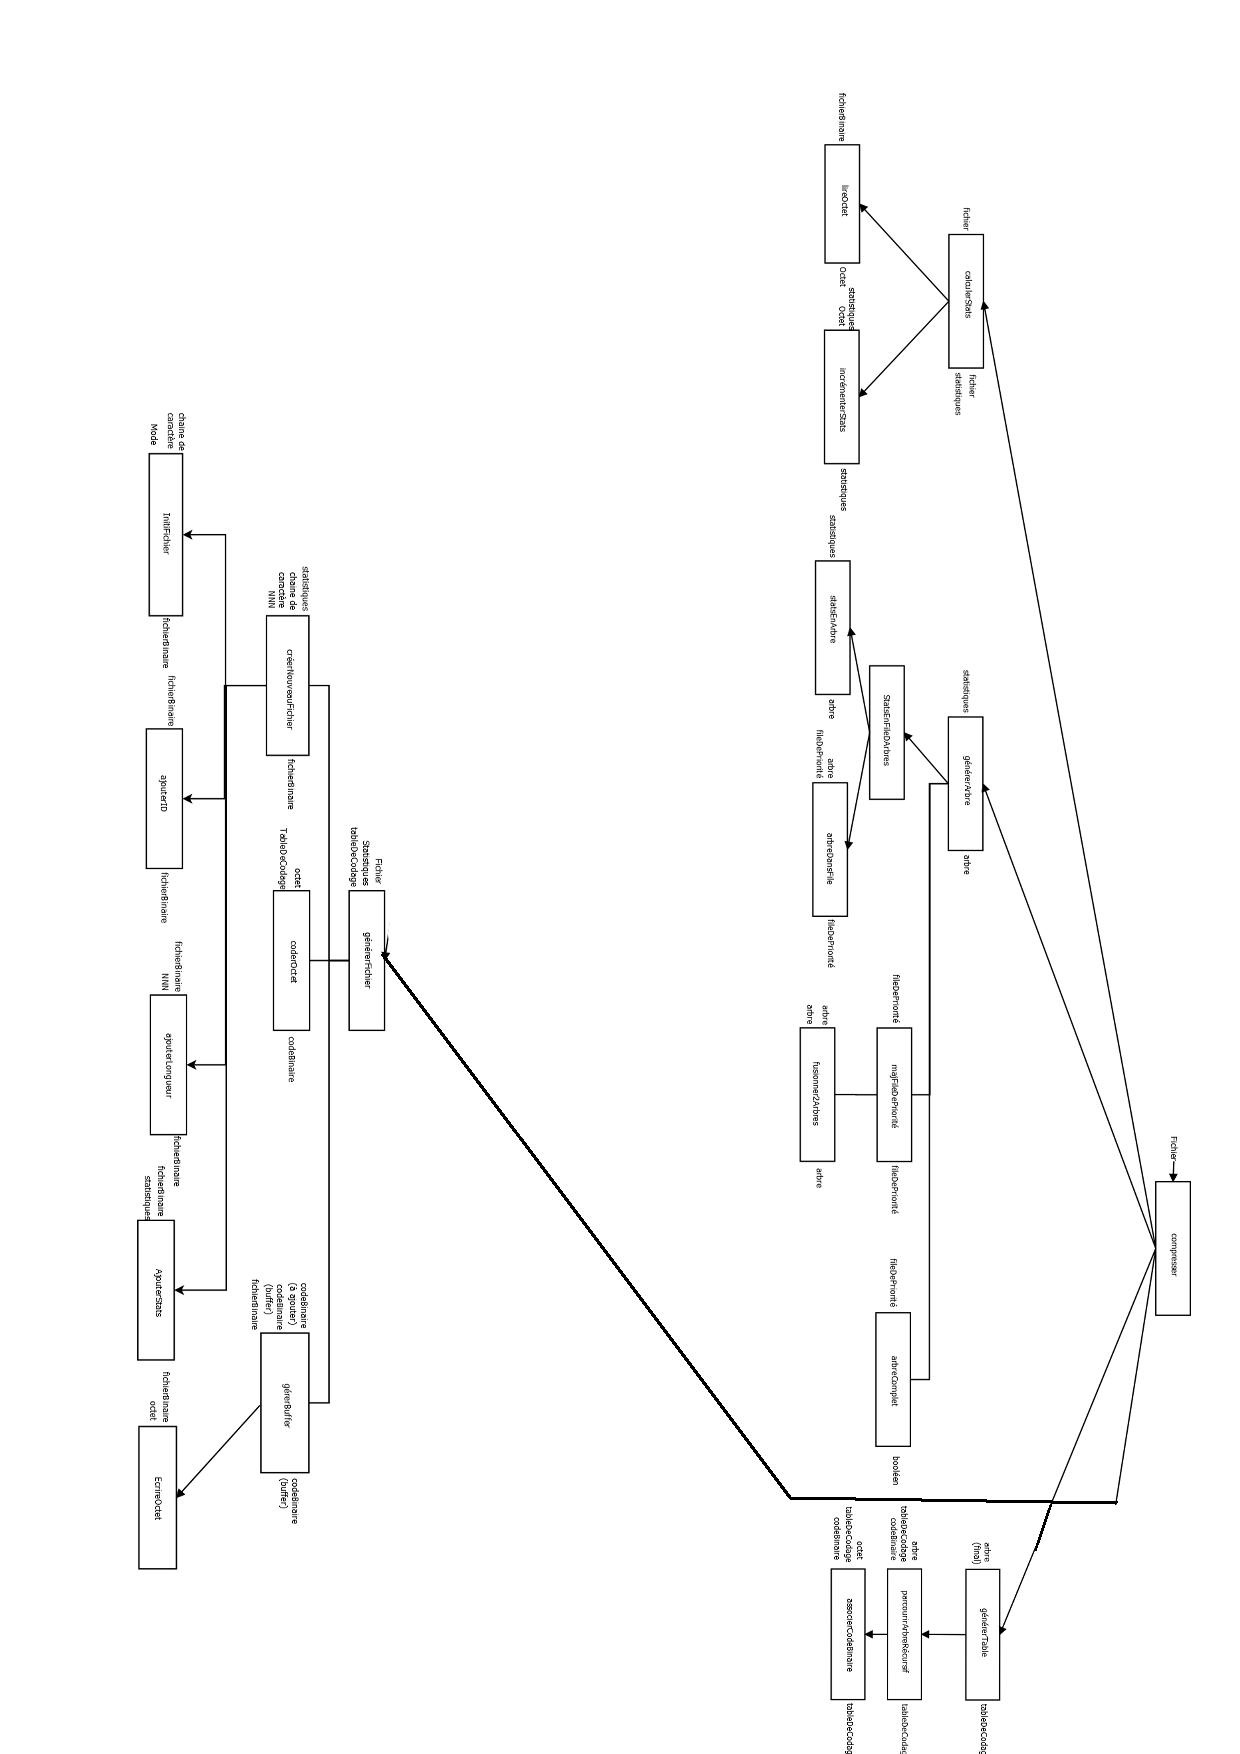
\includegraphics[width=0.7\textwidth]{images/compresser.pdf}

    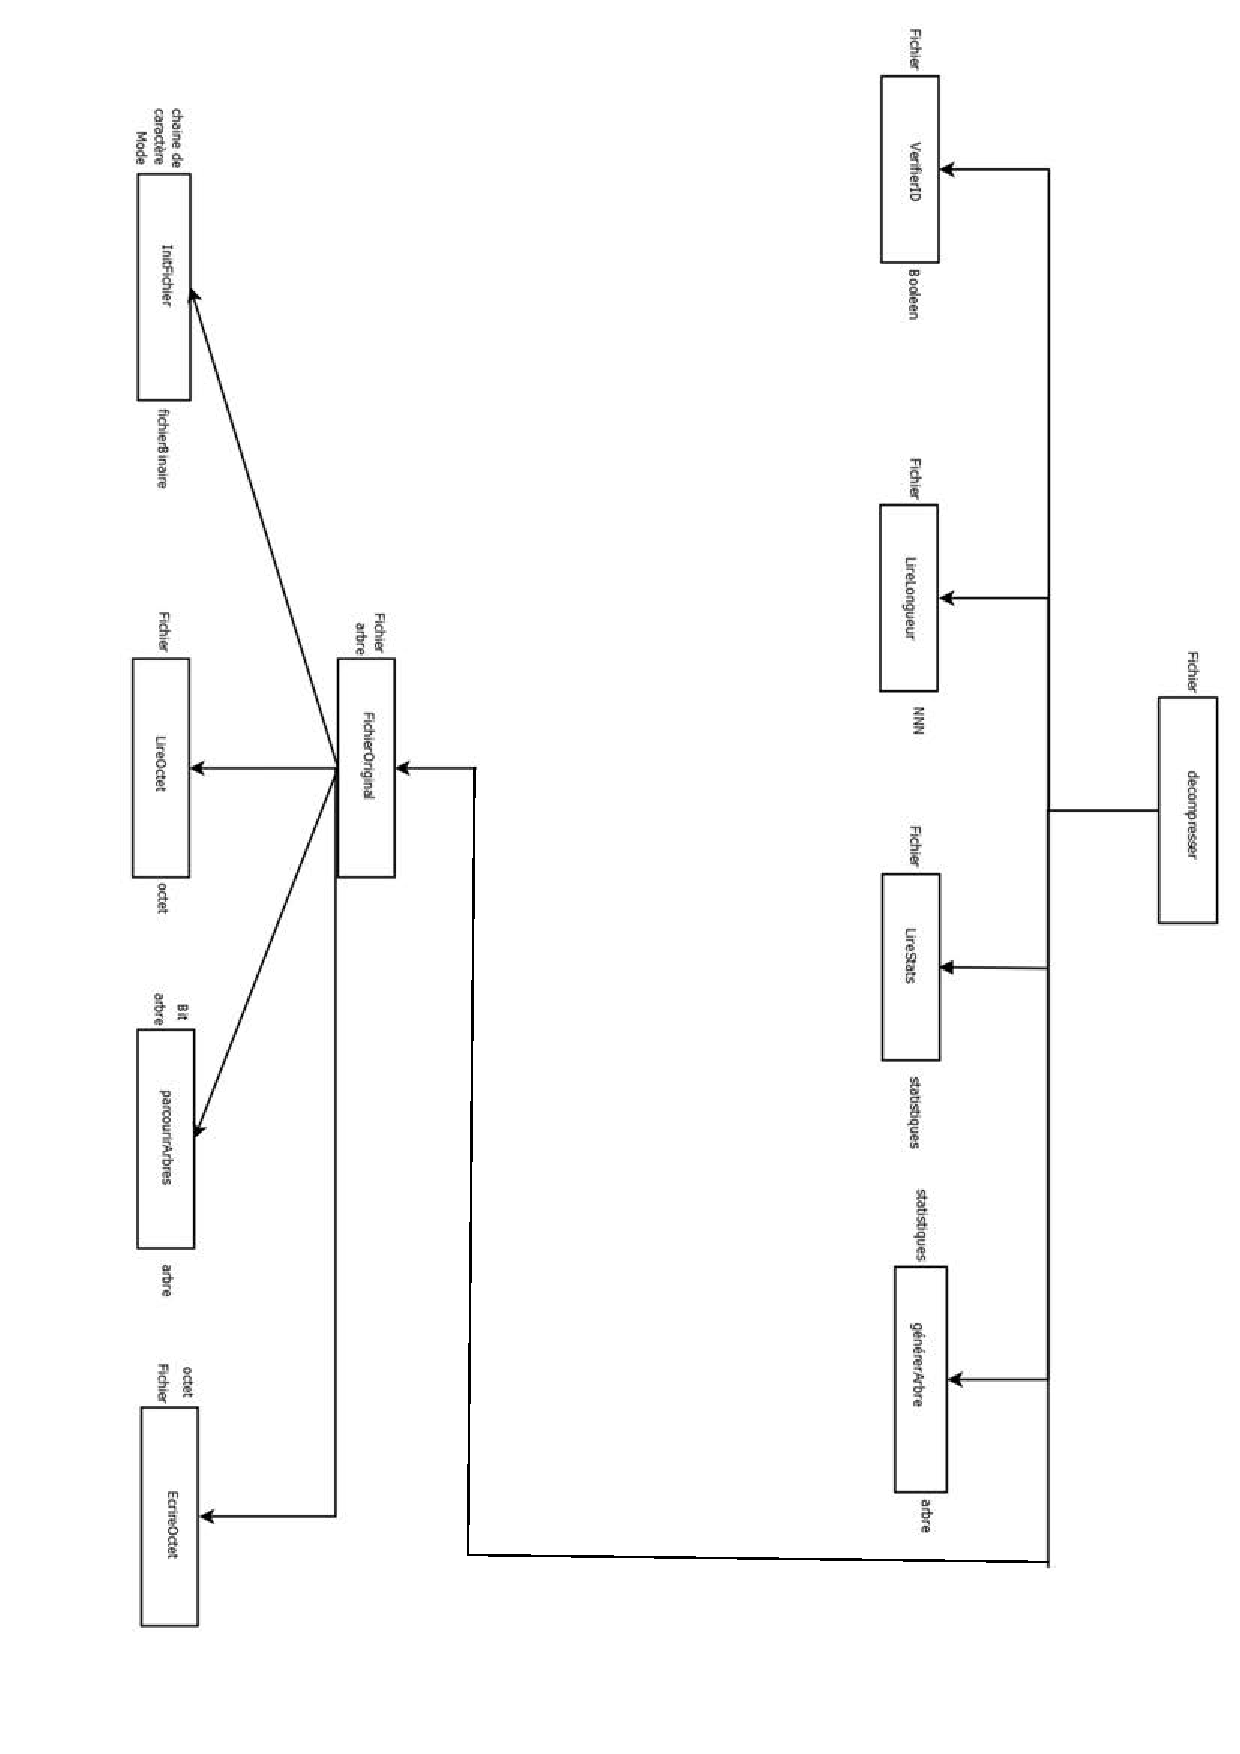
\includegraphics[width=0.8\textwidth]{images/decompresser.pdf}

\section{Conception des structures}
    %Une page d'introduction pour la conception detaillée
    Le contenu de cette section présente la conception des structures qui ont été mises en évidence dans la partie TAD.

    %Une page par TAD, en fichier PDF
    \clearpage

	    \section*{Arbre de Huffman}
    \subsection*{Conception préliminaire}
    \subsubsection*{Structure}

    Type ArbreDeHuffman = Structure
	\begin{itemize}[label=$\ $, leftmargin=2cm]
		 \item filsD, filsG : ArbreDeHuffman
		 \item poids : Naturel
		 \item octet : Octet 
	\end{itemize}
    finStructure
    
    \subsubsection*{Signatures}

	\begin{itemize}[label=$\ $, leftmargin=1cm]
		 \item \textbf{fonction} creerArbreDeHuffman():ArbreDeHuffman
		 \item \textbf{fonction} estVide(arbre:ArbreDeHuffman):Booleen
		 \item \textbf{fonction} estFeuille(arbre:ArbreDeHuffman):Booleen
		 \item \textbf{fonction} insérerRacine(poids:Naturel, fg, fd:ArbreDeHuffman) : ArbreDeHuffman
		 \begin{itemize}[label=$| $]
            \item \textbf{précondition:} non estVide(fg) et non estVide(fd)
         \end{itemize}
         \item \textbf{fonction} insérerFeuille(octet: Octet, poids:Naturel, fg,fd:ArbreDeHuffman): ArbreDeHuffman
         \begin{itemize}[label=$| $]
            \item \textbf{précondition:} estVide(fg) et estVide(fd)
         \end{itemize}
         \item \textbf{fonction} obtenirPoids(arbre:ArbreDeHuffman):Naturel
         \item \textbf{fonction} obtenirOctet(arbre:ArbreDeHuffman):Octet
         \begin{itemize}[label=$| $]
            \item \textbf{précondition:} estFeuille(arbre)
         \end{itemize}
         \item \textbf{fonction} obtenirFilsGauche(arbre:ArbreDeHuffman):ArbreDeHuffman
         \begin{itemize}[label=$| $]
            \item \textbf{précondition:} non estVide(arbre)
         \end{itemize}
         \item \textbf{fonction} obtenirFilsDroit(arbre:ArbreDeHuffman):ArbreDeHuffman
         \begin{itemize}[label=$| $]
            \item \textbf{précondition:} non estVide(arbre)
         \end{itemize}
         \item \textbf{fonction} comparer(arbre1, arbre2:ArbreDeHuffman):Booleen
         \item \textbf{procédure} supprimer(E/S arbre:ArbreDeHuffman)

	\end{itemize} 

    \subsection*{Conception détaillée}

    \begin{function}
    \SetAlgoLined
    \caption{creerArbreDeHuffman( ): ArbreDeHuffman}
    \Declaration{arbre: ArbreDeHuffman }
    \Deb{
        allouer(arbre) \\
       arbre.filsG$\gets$ NIL \\
       arbre.filsD$\gets$ NIL \\
        \Retour{arbre}
    }
    \end{function}

    \begin{function}
    \SetAlgoLined
    \caption{estVide( arbre: ArbreDeHuffman): Booleen}
    \Deb{
        \Retour{ (obtenirFilsGauche(arbre) = NIL) et (obtenirFilsDroit(arbre) = NIL)}
    }
    \end{function}

    \begin{function}
    \SetAlgoLined
    \caption{estFeuille( arbre: ArbreDeHuffman): Booleen}
    \Pre{non estVide(arbre)} \\
    \Deb{
        \Retour{ estVide(obtenirFilsGauche(arbre)) et estVide(obtenirFilsDroit(arbre))}
    }
    \end{function}

    \begin{function}
    \SetAlgoLined
    \caption{insererRacine(poids: Naturel, fg,fd: ArbreDeHuffman): ArbreDeHuffman}
    \Pre{non estVide(fg) et non estVide(fd)} \\
    \Declaration{arbre: ArbreDeHuffman }
    \Deb{
        allouer(arbre) \\
       arbre.filsG$\gets$ fg \\
       arbre.filsD$\gets$ fd \\
       arbre.poids $\gets$ poids \\
        \Retour{ arbre }
    }
    \end{function}

    \begin{function}
    \SetAlgoLined
    \caption{insererFeuille(octet: Octet, poids: Naturel, fg,fd: ArbreDeHuffman): ArbreDeHuffman}
    \Pre{estVide(fg) et estVide(fd)} \\
    \Declaration{arbre: ArbreDeHuffman }
    \Deb{
        allouer(a) \\
       arbre.filsG$\gets$ fg \\
       arbre.filsD$\gets$ fd \\
       arbre.poids $\gets$ poids \\
        arbre.octet $\gets$ octet \\
        \Retour{ a }
    }
    \end{function}

    \begin{function}
    \SetAlgoLined
    \caption{obtenirPoids(arbre: ArbreDeHuffman): Naturel}
    \Pre{ non estVide(arbre) } \\
    \Deb{
        \Retour{arbre.poids }
    }
    \end{function}
    
    \begin{function}
    \SetAlgoLined
    \caption{obtenirOctet( arbre: ArbreDeHuffman): Octet}
    \Pre{ estFeuille(arbre) } \\
    \Deb{
        \Retour{ arbre.octet }
    }
    \end{function}
    
    \begin{function}
    \SetAlgoLined
    \caption{obtenirFilsGauche( arbre: ArbreDeHuffman): ArbreDeHuffman}
    \Deb{
        \Retour{ arbre.filsG }
    }
    \end{function}

    \begin{function}
    \SetAlgoLined
    \caption{obtenirFilsDroit( arbre: ArbreDeHuffman): ArbreDeHuffman}
    \Deb{
        \Retour{ arbre.filsD }
    }
    \end{function}
    
    \begin{procedure}
    \SetAlgoLined
    \caption{supprimer(E/S arbre: ArbreDeHuffman)}
    \Declaration{tmp: ArbreDeHuffman}
    \Deb{
        \If{ non estVide(arbre) }{
            tmp $\gets$ obtenirFilsGauche(arbre) \\
            supprimer(tmp) \\
            tmp $\gets$ obtenirFilsDroite(arbre) \\
            supprimer(tmp) \\
        }
        liberer(arbre)
    }
    \end{procedure}
    \clearpage
    
	    \section*{CodeBinaire}

    Le code binaire est constitué de bit, nous avons décidé de représenter le code binaire comme une structure contenant un tableau de bit ainsi qu'un naturel qui nous permettra de connaître la longueur du tableau qui est occupée :

    \subsection*{Conception préliminaire}
    \subsubsection*{Structure}

	
    Type Bit = Naturel \{0,1\} \\
    Type CodeBinaire = Structure
	\begin{itemize}[label=$\ $, leftmargin=2cm]
	    \item code : Tableau [1...MAX] de Bit
	    \item longueur : Naturel
    \end{itemize}
	finstructure

    \subsubsection*{Signatures}

    \begin{itemize}[label=$\ $, leftmargin=1cm]
        \item \textbf{fonction} creerCodeBinaire( ) : CodeBinaire
        \item \textbf{fonction} longueur(cBinaire : CodeBinaire) : Naturel
        \item \textbf{fonction} iemeBit (cBinaire : CodeBinaire, iemePlace : Naturel) : Bit
        \begin{itemize}[label=$| $, leftmargin=1cm]
            \item \textbf{précondition} : 0 $<$ iemePlace et iemePlace $ \leqslant$ longueur(cBinaire)
        \end{itemize}
        \item \textbf{procédure} ajouterBit(E/S cBinaire : CodeBinaire, E bit : Bit)
        \begin{itemize}[label=$| $, leftmargin=1cm]
            \item \textbf{précondition} : longueur(cBinaire) $<$ 256
        \end{itemize}
        \item \textbf{procédure} modifierIemeBit (E/S cBinaire : CodeBinaire, E iemePlace : Naturel, bit : Bit)
        \begin{itemize}[label=$| $, leftmargin=1cm]
            \item \textbf{précondition} : 0 $<$ iemePlace et iemePlace $ \leqslant$ longueur(cBinaire)
        \end{itemize}
        \item \textbf{procédure} supprimerIemeBit (E/S cBinaire : CodeBinaire, E iemePlace : Naturel)
        \begin{itemize}[label=$| $, leftmargin=1cm]
            \item \textbf{précondition} : 0 $<$ iemePlace et iemePlace $ \leqslant$ longueur(cBinaire)
        \end{itemize}
        \item \textbf{fonction} sontEgaux(cBinaire1, cBinaire2 : CodeBinaire) : Booleen
    \end{itemize}

    \subsection*{Conception détaillée}
    
    \begin{function}[H]
    \SetAlgoLined
    \Deb
        {$resultat.longueur \gets 1$ 
        $resultat.code[1] \gets 0$ 
        \Retour{resultat}}
    \caption{creerCodeBinaire( ):CodeBinaire}
    \end{function}

    \begin{function}
    \SetAlgoLined
    \caption{longueur(cBinaire:CodeBinaire):Naturel} 
    \Deb{
        \Retour{cBinaire.longueur}}
    \end{function}

    \begin{function}
    \SetAlgoLined
    \caption{iemeBit (cBinaire:CodeBinaire, iemePlace : Naturel) : Bit} 
    \Pre{(0 $<$ iemePlace) et (iemePlace $\leq$ longueur(cBinaire))} \\
    \Deb{
        \Retour{cBinaire.code[iemePlace]}}
    \end{function}

    \begin{procedure}
    \SetAlgoLined
    \caption{ajouterBit(E/S cBinaire:CodeBinaire,E bit:Bit)}
    \Deb
        {$cBinaire.longueur \gets longueur(cBinaire)+1$ 
        $cBinaire.code[longueur(cBinaire)] \gets bit$ 
        }
    \end{procedure}

    \begin{procedure}
    \SetAlgoLined
    \caption{modifierIemeBit(E/S:cBinaire:CodeBinaire,E:iemePlace:Naturel,bit:Bit)}
    \Pre{(0 $<$ iemePlace) et (iemePlace $\leq$ longueur(cBinaire))} \\
    \Deb
        {$cBinaire.code[iemePlace] \gets bit$ 
        }
    \end{procedure}

    \begin{procedure}
    \SetAlgoLined
    \caption{supprimerIemeBit(E/S:cBinaire:CodeBinaire,E:iemePlace:Naturel)}
    \Pre{(0 $<$ iemePlace) et (iemePlace $\leq$ longueur(cBinaire))} \\
    \Declaration{i:Naturel }
    \Deb
        {\Pour{$i \gets iemePlace+1$ \KwA longueur(cBinaire)}{modifierIemeBit(cBinaire, i-1, iemeBit(cBinaire,i))}
        $cBinaire.longueur \gets longueur(cBinaire)-1$ 
        }
    \end{procedure}

    \begin{function}
    \SetAlgoLined
    \caption{sontEgaux(cBinaire1,cBinaire2:CodeBinaire):Booleen} 
    \Declaration{egaux: Booleen }
    \Deb{
        $egaux \gets Vrai$ 
        \Si{$longueur(cBinaire1) \neq longueur(cBinaire2) $}{$egaux \gets Faux$ }
        \Tq{(i $\leq$ longueur(cBinaire1) et egaux)}{
            \Si{iemeBit(cBinaire1,i) $\neq$ iemeBit(cBinaire2,i)}{$egaux \gets Faux$ }
        $i \gets i+1$}}
        \Retour{egaux}
    \end{function}


    \begin{function}
    \SetAlgoLined
    \caption{codebinaireEnOctet(cBinaire: CodeBinaire)}
    \Pre{longueur(cBinaire) $\leq$ 8} \\
    \Declaration{octet:Octet, i:Entier}
    \Deb{
    $octet \gets creeroctet()$
    \Pour{$i \gets 1$ \KwA longueur(cBinaire)}{ecrireIemeBit(octet,9-i,iemeBit(cBinaire,i)}}
    \Retour{octet}
    \end{function}
    \clearpage
    
	    \section*{FileDePriorite}
    \subsection*{Conception préliminaire}
    \subsubsection*{Structure}
 
    Type ListeChaineeArbre = ListeChainee$<$Arbre$>$ (resp. Noeud$<$Arbre$>$)
 
    Type FileDePriotrite = Structure
	\begin{itemize}[label=$\ $, leftmargin=2cm]
		 \item debut : ListeChaineeArbre
		 \item fin : ListeChaineeArbre
	\end{itemize}
 
    finStructure
 
	\subsubsection*{Signatures}
	
    \begin{itemize}[label=$\ $, leftmargin=1cm]
        \item \textbf{fonction} obtenirDebut (file : FileDePriorite) : ListeChaineeArbre
        \item \textbf{fonction} obtenirFin (file:FileDePriorite) : ListeChaineeArbre
        \item \textbf{procédure} fixerDebut (E/S file : FileDePriorite, E debut : ListeChaineeArbre)
        \item \textbf{procédure} fixerFin(E/S file : FileDePriorite, E fin : ListeChaineeArbre)
        \item \textbf{fonction} obtenirElementListe (liste : ListeChaineeArbre) : ArbreDeHuffman
        \item \textbf{procédure} fixerElementListe (E/S liste : ListeChaineeArbre, E arbre : ArbreDeHuffman)
        \item \textbf{fonction} listeEstVide (liste : ListeChaineeArbre) : Booleen
        \item \textbf{fonction} creerFile ( ) : FileDePriorite
        \item \textbf{fonction} EstVide (file:FileDePriorite) : Booleen
        \item \textbf{procédure} enfiler (E/S file :  FileDePriorite, E arbre : ArbreDeHuffman)
        \item \textbf{procédure} defiler (E/S file :  FileDePriorite)
        \item \textbf{fonction} obtenirArbre (file:FileDePriorite) :ArbreDeHuffman
    \end{itemize} 
    

    \subsection*{Conception détaillée}
 
    \begin{function}
    \SetAlgoLined
    \caption{obtenirDebut(file : FileDePriorite) : ListeChaineeArbre}
    \Deb{
        \Retour{file.debut}
        }
    \end{function}
 
    \begin{function}
    \SetAlgoLined
    \caption{obtenirFin(file : FileDePriorite) : ListeChaineeArbre}
    \Deb{
        \Retour{file.fin}
        }
    \end{function}
 
    \begin{procedure}
    \SetAlgoLined
    \caption{fixerDebut(E/S file : FileDePriorite, E debut : ListeChaineeArbre)}
    \Deb{
        file.debut $\gets$ debut \\
        }
    \end{procedure}
 
    \begin{procedure}
    \SetAlgoLined
    \caption{fixerFin(E/S file : FileDePriorite, E fin : ListeChaineeArbre)}
    \Deb{
        file.fin $\gets$ fin² \\
        }
    \end{procedure}
 
    \begin{function}
    \SetAlgoLined
    \caption{obtenirElementListe(liste : ListeChaineeArbre): ArbreDeHuffman}
    \Deb{
        \Retour{file.fin}
        }
    \end{function}
 
    \begin{procedure}
    \SetAlgoLined
    \caption{fixerElementListe(E/S liste : ListeChaineeArbre, E arbre : ArbreDeHuffman)}
    \Deb{
        liste.arbre $\gets$ arbre
        }
    \end{procedure}
 
    \begin{function}
    \SetAlgoLined
    \caption{listeEstVide(liste : ListeChaineeArbre) : Booleen}
    \Deb{
        \Retour{liste.arbre=NIL}
        }
    \end{function}
 
    \begin{function}
    \SetAlgoLined
    \caption{creerFile ( ) : FileDePriorite}
    \Declaration{file : FileDePriorite }
    \Deb{
        fixerDebut(file,NIL)\\
        fixerFin(file,NIL)\\
        \Retour{file}
        }
    \end{function}
 
    \begin{function}
    \SetAlgoLined
    \caption{EstVide(file:FileDePriorite) :  Booleen}
    \Deb{
        \Retour{ obtenirDebut(file) = NIL}
    }
    \end{function}
 
    \begin{procedure}
    \SetAlgoLined
    \caption{enfiler (E/S file :  FileDePriorite, E arbre : ArbreDeHuffman)}
    \Declaration{tmp, noeud: ListeChainee, fin: Booleen}
    \Deb{
        allouer(tmp) \\
        fixerElementListe(tmp,arbre) \\
        \Si{estVide(file)}{
            fixerDebut(file,tmp)\\
            fixerFin(file,tmp)\\
        }
        \Si{
            comparer(obtenirElementListe(tmp),obtenirArbre(file)) $<$ 0
        }{
            LC\_fixerListeSuivante(tmp,obtenirDebut(file))\\
            fixerDebut(file,tmp)
        }
        \Sinon{
            fin $\gets$ faux\\
            noeud $\gets$ obtenirDebut(file)\\
            \Tq{non(fin)}{
                \Si{listeEstVide(LC\_obtenirListeSuivante(noeud))}{
                    LC\_fixerListeSuivante(noeud,tmp)\\
                    fixerFin(file,tmp)\\
                    fin $\gets$ true\\
                    }
                \Si {comparer(obtenirElementListe(tmp),obtenirElementListe(LC\_obtenirListeSuivante(noeud)))$<$0)}{
                    LC\_fixerListeSuivante(tmp,LC\_obtenirListeSuivante(noeud))\\
                    LC\_fixerListeSuivante(noeud,tmp)\\
                    fin $\gets$ true\\
                }
                \Sinon{ noeud $\gets$ LC\_obtenirlisteSuivante(noeud) }
            }
            }
    }
    \end{procedure}
 
    \begin{procedure}
    \SetAlgoLined
    \caption{defiler (E/S file :  FileDePriorite)}
    \Declaration{tmp: ListeChaineeArbre}
    \Deb{
        tmp $\gets$ obtenirDebut(file)\\
 
        \Si{non(listeEstVide(LC\_obtenirListeSuivante(obtenirDebut(\^{}file))))}{
            fixerDebut(file,LC\_obtenirListeSuivante(obtenirDebut(\^{}file)))\\
        }
        \Sinon{
            fixerDebut(file,NIL )\\
            fixerFin(file,NIL) \\ 
        }
 
        liberer(tmp)
    }
    \end{procedure}
 
    \begin{function}
    \SetAlgoLined
    \caption{obtenirArbre (file : FileDePriorite) : ArbreDeHuffman}
    \Deb{
 
        \Retour{file.debut\^{}.arbre}
 
    }
    \end{function}
    \clearpage
    
	    \section*{Octet}
    \subsection*{Conception préliminaire}
    \subsubsection*{Structure}

    Type Octet = tableau [1..8] de Bit

    \subsubsection*{Signatures}
    \begin{itemize}[label=$\ $, leftmargin=1cm]
         \item \textbf{fonction} creerOctet (S: Octet)
         \item \textbf{procédure} ecrireIemeBit (E/S o : Octet, E i : Naturel, b : Bit)
            \begin{itemize}[label=$| $, leftmargin=1cm]
                \item \textbf{précondition} : 1 $\leq$ i $\leq$ 8
            \end{itemize}
        \item \textbf{fonction} lireIemeBit (o : Octet, i : Naturel) :Bit
            \begin{itemize}[label=$| $, leftmargin=1cm]
                \item \textbf{précondition} : 1 $\leq$ i $\leq$ 8
            \end{itemize}
        \item \textbf{fonction} sontEgaux (o1, o2 : Octet) : Booleen
    \end{itemize}

    \subsection*{Conception détaillée}

    \begin{function}
    \SetAlgoLined
    \caption{creerOctet( ):Octet}
    \Declaration{o:Octet, i:Naturel}
    \Deb {
        \Pour{$i \gets 1$ \KwA 8}{
        $o[i] \gets 0$ 
        }
        \Retour{o}
        }
    \end{function}

    \begin{procedure}
    \SetAlgoLined
    \caption{ecrireIemeBit (E/S o : Octet, E i : Naturel, b : Bit)}
    \Pre{i $\geq$ 1 et i $\leq$ 8} \\
    \Deb {
        $o[i] \gets b$ 
        }
    \end{procedure}

    \begin{function}
    \SetAlgoLined
    \caption{lireIemeBit (o : Octet, i : Naturel) :Bit}
    \Pre{i $\geq$ 1 et i $\leq$ 8} \\
    \Deb {
        \Retour{o[i]}
        }
    \end{function}

    \begin{function}
    \SetAlgoLined
    \caption{sontEgaux (o1, o2 : Octet) : Booleen}
    \Declaration{i:Naturel, egaux:Booleen}
    \Deb {
        $egaux \gets Vrai$ 
        $i \gets 1$ 
        \Tq{i $\leq$ 8 et egaux}{
            \Si{o1[i] $\neq$ o2[i]}{
                $egaux \gets Faux$
                }
            $i \gets i+1$ 
        }
        \Retour{egaux}
        }
    \end{function}
    \clearpage
    
	    \section*{Statistiques}
    On a ici un dictionnaire (clé: Octet, valeur: Naturel). On va donc utiliser une fonction de hash
    \subsection*{Conception préliminaire}
    \subsubsection*{Structure}

    Type Statistiques= Tableau [1..256] de Naturel 

    \subsubsection*{Signatures}
    \begin{itemize}[label=$\ $, leftmargin=1cm]
        \item \textbf{fonction} hash(o:Octet):Naturel
        \item \textbf{fonction} statistiques(): Statistiques
        \item \textbf{procédure} ajouterOctet(E/S stat:Statistiques, E octet:Octet, nbOccur:Naturel)
        \begin{itemize}[label=$| $, leftmargin=1cm]
            \item \textbf{précondition} : non estPresent(stat,octet)
        \end{itemize}
        \item procedure modifierOctet(E/S stat:Statistiques, E octet:Octet, nbOccur:Naturel)
        \begin{itemize}[label=$| $, leftmargin=1cm]
            \item \textbf{précondition} : estPresent(stat,octet)
        \end{itemize}
        \item \textbf{fonction} nbElements( stat: Statistiques): Naturel
        \item \textbf{fonction} estVide (stat: Statistiques) : Booléen
        \item \textbf{fonction} estPresent( stat: Statistiques, octet: Octet): Booléen
        \item \textbf{fonction} obtenirOccurence( stat: Statistiques, octet: Octet): Naturel
        \item \textbf{procédure} supprimerOctet(E/S stat: Statistiques, E octet:Octet)
        \begin{itemize}[label=$| $, leftmargin=1cm]
            \item \textbf{précondition} : estPresent(stat,octet)
        \end{itemize}
        \item \textbf{procédure} obtenirClefs(E stat:Statistiques, S clefs: Liste $<$Octet$>$)
	\end{itemize} 


    \subsection*{Conception détaillée}
    
    \begin{function}
        \SetAlgoLined
        \caption{hash(o:Octet): Naturel} 
        \Deb{
        \Retour{OctetEnNaturel(o)}} 00 on obtient 0, FF on obtient 255
    \end{function}

    \begin{function}
        \SetAlgoLined
        \caption{statistiques( ) :  Statistiques} 
        \Declaration \\
            i : Naturel\\
            stat:Statistiques\\
        \Deb{
        \Pour {i $\gets$ 1 a 256} {stat[i] $\gets$ 0}
        \Retour{stat}}
    \end{function}

        
    \begin{procedure}
        \SetAlgoLined
        \caption{ajouterOctet(E/S stat:Statistiques,E octet:Octet,nbOccur:Naturel)}
        \Pre{non(estPresent(stat,octet))} \\
        \Deb{
        stat[hash(octet)] $\gets$ nbOccur }
    \end{procedure}
        
    \begin{procedure}
        \SetAlgoLined
        \caption{modifierOctet(E/S stat:Statistiques, E octet:Octet, E nbOccur:Naturel)}
        \Pre{estPresent(stat,octet))} \\
        \Deb{
        stat[hash(octet)] $\gets$ nbOccur }
    \end{procedure}

    \begin{function}
        \SetAlgoLined
        \caption{nbElements( stat:  Statistiques):Naturel} 
        \Declaration\ i,taille : Naturel\\
        \Deb{
        taille $\gets$ 1\\
        \Pour {i $\gets$ 1 a 256} {\Si{non(stat[i]=0)}{taille$\gets$taille+1}}
        \Retour{taille}}
    \end{function}

    \begin{function}
        \SetAlgoLined
        \caption{EstVide( stat:  Statistiques):Booleen} 
        \Deb{
        
        \Retour{nbElements(stat)=0}}
    \end{function}


    \begin{function}
        \SetAlgoLined
        \caption{EstPresent( stat:  Statistiques,octet:Octet):Booleen} 
        \Deb{
        \Retour{obtenirOccurence(stat,octet)!=0)}}
    \end{function}

    \begin{function}
        \SetAlgoLined
        \caption{obtenirOccurence( stat:  Statistiques,octet:Octet):Naturel} 
        \Deb{
        \Retour{stat[hash(octet)]}}
    \end{function}

    \begin{procedure}
        \SetAlgoLined
        \caption{supprimerOctet(E/S stat:Statistiques,E octet:Octet)}
        \Pre{estPresent(stat,octet)} \\
        \Deb{
        modifierOctet(stat,octet,0)}
    \end{procedure}

    \begin{procedure}
        \SetAlgoLined
        \caption{obtenirClefs(E stat:Statistiques,S clefs: Liste $<$Octet$>$)}
        \Declaration\ i : Naturel\\
        \Deb{
        //Notre fonction de hash est bijective on parcours tout le tableau \\ pour trouver de clefs ayant une statistique non nulle//\\
        \Pour {i $\gets$ 1 a 256} 
        {\Si{stat[i]$>$0}{Liste$\_$ajouter(clefs,naturelEnOctet(i))}}}
    \end{procedure}

    \clearpage
    
	    \section*{TableDeCodage}
Pour la conception de la table de codage, on observe avec le TAD que l’on doit concevoir un dictionnaire. (Avec un octet en clé, et un code binaire en valeur). On a donc considéré les éléments suivants : \\

        	- On veut une recherche de la clé rapide (en O(1) si possible, O(log n) sinon), en effet, durant la phase de compression du fichier, on va  faire une recherche pour chaque octet du fichier source (de l’ordre du Mo, $ ~= 10^6 $ recherches). \\
            
            - L'utilisation de la mémoire doit rester raisonnable (cad éviter de stocker des clés sans valeurs), cependant, on sait que nos clés sont des Octets (1 octet), et nos valeurs des Codes binaires (8 bits maximum). L’utilisation d’un tableau représente donc : 
            
	$$ taille_{tableau} = nb_{cle} * taille_{valeur} $$
	$$ taille_{tableDeCodage} = 256 * taille_{octet} = 256 * 1 = 256 $$

    Notre table de codage va donc être un tableau, et on aura une fonction pour transformer un octet en indice de ce tableau: \\
    
    \subsection*{Conception préliminaire}
    \subsubsection*{Structure}
        TableDeCodage = tableau[1..256] de CodeBinaire

    \subsubsection*{Signatures}
	\begin{itemize}[label=$\ $, leftmargin=1cm]
		\item \textbf{fonction} hash(o: Octet) : [1..256]
		\item \textbf{fonction} creerTableDeCodage() : TableDeCodage
		\item \textbf{procedure} ajouterOctet(E/S tdc: TableDeCodage, E octet: Octet, code: CodeBinaire)
		\begin{itemize}[label=$| $]
			\item \textbf{précondition:} non elementPresent(tdc, octet)
		\end{itemize}
		\item \textbf{procedure} supprimerOctet(E/S tdc: TableDeCodage, E octet: Octet)
		\begin{itemize}[label=$| $]
			\item \textbf{précondition:} octetPresent(tdc, octet)
		\end{itemize}
		\item \textbf{fonction} recupererCodeBinaire(tdc: TableDeCodage, octet: Octet): CodeBinaire
		\begin{itemize}[label=$| $]
			\item \textbf{précondition:} elementPresent(tdc, octet)
		\end{itemize}
		\item \textbf{fonction} estVide(tdc: TableDeCodage): Booleen
		\item \textbf{fonction} octetPresent(tdc: TableDeCodage, octet: Octet): Booleen
		\item \textbf{fonction} nbOctets(tdc: TableDeCodage): Naturel
	\end{itemize}

    \subsection*{Conception détaillée}
    
    \begin{function}
        \SetAlgoLined
        \caption{hash(o : Octet ) :  Naturel} 
        \Deb{
            \Retour{OctetEnNaturel(o)} //00 on obtient 0, FF on obtient 255
        }
    \end{function}
    
    \begin{function}
        \SetAlgoLined
        \caption{creerTableDeCodage( ):TableDeCodage}
        \Declaration{i : Naturel, tdc:TableDeCodage}
        \Deb{
            \Pour {i $\gets$ 1 a 256} {
                tdc[i] $\gets$ CreerCodeBinaire()
            }
            \Retour{tdc}
        }
    \end{function}
        
    \begin{procedure}
        \SetAlgoLined
        \caption{ajouterOctet(E/S tdc:TableDeCodage,E o:Octet, code:CodeBinaire)}
        \Pre{non(elementPresent(tdc,octet))} \\
        \Deb{ 
            tdc [hash(octet)] $\gets$ CodeBinaire
        }
    \end{procedure}
        
    \begin{procedure}
        \SetAlgoLined
        \caption{supprimerOctet(E/S tdc:tableDeCodage,E octet:Octet)}
        \Pre{OctetPresent(tdc,octet)} \\
        \Deb{
            ajouterOctet(tdc,octet,CreerCodeBinaire())
        }
    \end{procedure}
        
    \begin{function}
        \SetAlgoLined
        \caption{RecupererCodeBinaire(tdc: TabldeDeCodage,octet:Octet):Naturel} 
        \Pre{elementPresent(tdc,octet))} \\    
        \Deb{
            \Retour{tdc[hash(octet)]}
        }
    \end{function}
        
    \begin{function}
        \SetAlgoLined
        \caption{EstVide( tdc: TableDeCodage):Booleen } 
        \Declaration{i : Naturel, EstVide :Booleen}
        \Deb{
            i $\gets$ 1 \\
            EstVide $\gets$ Vrai \\
            \Tq {EstVide et i $\leq$ 256} {
                \Si {non(tdc[i]=0)} {
                    EstVide$\gets$Faux
                }
                i $\gets$i+1
            }
            \Retour{EstVide}
        }
    \end{function}

    \begin{function}
        \SetAlgoLined
        \caption{OctetPresent( tdc :  TableDeCodage,octet:Octet):Booleen} 
        \Deb{
            \Retour{non (RecupererCodeBinaire(tdc,octet)=0))}
        }
    \end{function}

    \begin{function}
        \SetAlgoLined
        \caption{nbElements( tdc:  TableDeCodage):Naturel} 
        \Declaration{i,resultat : Naturel}
        \Deb{
            \Pour {i $\gets$ 1 a 256}{
                \Si{non(tdc[i]=0)}{
                    resultat$\gets$resultat+1
                }
            }
            \Retour{resultat}
        }
    \end{function}

\clearpage % Pour faire un saut de page propre

\section{Conception Détaillée Métier}
    %TODO: Conception Detaillée

    Lorsque nous avons les outils permettant de manipuler nos données, il est temps de créer les fonctions et procédures qui permettront de les utiliser afin d'obtenir le résultat souhaité. Ainsi nous avons réfléchi aux principales fonctionnalités qui permettent de compresser ou décompresser.

    Le contenu de cette section présente la conception des structures qui ont été mises en évidence
\subsection*{Conception préliminaire:}
\begin{itemize}[label=$\ $, leftmargin=2cm]
    \item calculerStats(E/S fichier: Fichier, stats: Statistiques) 
    \item genererArbre(stats : Statistiques) : ArbreDeHuffman 
    \item majFileDePriorite(E/S file : FileDePriorite) 
    \item parcourirArbreR(E/S:tdc:TableDeCodage,E:arbre:ArbreDeHuffmann, code:codeBinaire) 
    \item gererBuffer(E code: CodeBinaire, E/S buffer: CodeBinaire, fichier: fichierBinaire) 
    \item FichierOriginal(E/S f : fichier, E a:ArbreDeHuffman) 
    \item Compresser(E FichierD: Fichier) 
    \item Decompresser(E FichierD: Fichier; S erreurFichier:Booleen)
\end{itemize}

\subsection*{Conception détaillée:}
%calculerStats
\begin{procedure}
    \SetAlgoLined
    \caption{calculerStats(E/S fichier: Fichier, stats: Statistiques)}
    \Declaration{
        octet: Octet \\
    }
    \Deb{
        \Tq{non finFichier(fichier.fb)}{
            octet $\gets$ lireOctet(fichier.fb) \\
            fichier.longueur = fichier.longueur + 1; \\
            incrementerStats(stats, octet)
        }
    }
\end{procedure}


%genererArbre
\begin{function}
    \SetAlgoLined
    \caption{genererArbre(stats : Statistiques) : ArbreDeHuffman}
    \Declaration{file : FileDePriorite, arbreFinal : ArbreDeHuffman}
    \Deb{
        file $ \gets $ statsEnFileDArbre(stats) \\
        \Tq{ non(arbreComplet(file)) }{
            majFileDePriorite(file)
        }
        arbreFinal $\gets$ obtenirArbre(file) \\
        defiler(file) \\
        \Retour{arbreFinal}
    }
\end{function}

%majFileDePriorite
    \begin{procedure}
    \SetAlgoLined
    \caption{majFileDePriorite(E/S file : FileDePriorite)}
    \Declaration{a1,a2,arbreFusion : ArbreDeHuffman}
    \Deb{
        a1 $ \gets $ obtenirArbre(file) \\
        defiler(file) \\
        a2 $ \gets $ obtenirArbre(file) \\
        defiler(file) \\
        arbreFusion $ \gets $ fusionner2Arbres(a1,a2)\\
        enfiler(file,arbreFusion)\\
        }
    \end{procedure}


%genererTable
%parcourirArbreRecursif
    \begin{procedure}
    \SetAlgoLined
    \caption{parcourirArbreR(E/S:tdc:TableDeCodage,E:arbre:ArbreDeHuffmann, code:codeBinaire)}
    \Deb{
    \Si{estFeuille(arbre)}{associerCodeBinaire(tdc,code,obtenirElement(arbre))\;}
	\Sinon{
	ajouterBit(code,0)\;
	parcourirArbreR(tdc,(obtenirFilsGauche(arbre),code)\;
	modifierIemeBit(code, longueur(code), 1)\;
    	parcourirArbreR(tdc,(obtenirFilsDroit(arbre),code)\;}}
    \end{procedure}
    
    \begin{function}
    \SetAlgoLined
    \caption{genererTable(arbreFinal:ArbreDeHuffmann):TableDeCodage}
    \Declaration {tdc: TableDeCodage }
    \Deb
    {tdc$\gets$creerTableDeCodage( )\;
    parcourirArbreR(tdc,arbreFinal,creerCodeBinaire( ))\;
    \Return { tdc }
     }
    \end{function}


%genererFichier
%gererBuffer
    \begin{procedure}
    \SetAlgoLined
    \caption{gererBuffer(E code: CodeBinaire, E/S buffer: CodeBinaire, fichier: fichierBinaire)}
    \Declaration{i: Naturel}
    \Deb{
    	\Pour{i $\gets$ 1 \KwA longueur(code) }{
    		ajouterBit(buffer, iemeBit(code, i)) \\
    		\Si{longueur(buffer) = 8}{
    			EcrireOctet(fichier, codeBinaireEnOctet(buffer)) \\
                buffer = creerCodeBinaire() \\
    		}
    	}
    }
    \end{procedure}
    
    \begin{function}
    \SetAlgoLined
    \caption{codeBinaireEnOctet(code): octet}
    \Declaration{
        o: Octet \\
	    i: Naturel \\
    }
    \Deb{
    	\Pour{i $\gets$ 1 \KwA 8 }{
            changerIeme(octet, i, iemeBit(code, j))
    	}
    	
    	\Return octet
    }
    \end{function}
    
    \begin{procedure}
    \SetAlgoLined
    \caption{genererFichier(E stats: Statistiques, tdc: TableDeCodage, fOriginal: fichierBinaire, nomOriginal: CDC)}
    \Declaration{
    fCompr: fichierBinaire \\
	codeB, buffer: CodeBinaire \\
    }
    \Deb{
    	creerNouveauFichier(fCompr, stats, nomOriginal, longueur(fOriginal)) \\
    
        buffer = creerCodeBinaire()
    	\Tq{non finFichier(fOriginal)}{
    		codeB $\gets$ coderOctet(tdc, lireOctet(fOriginal)) \\
    		gererBuffer(codeB, buffer, fichierOriginal) \\
    	}
    	
    	\Si{longueur(buffer) $\neq$ 0}{
    		ecrireOctet(fCompr, codeBinaireEnOctet(buffer))
    	}
    	
    	fermer(fCompr) \\
    }
    \end{procedure}


%fichierOriginal
 \begin{procedure}
    \SetAlgoLined
    \caption{FichierOriginal(E/S f : fichier, E a:ArbreDeHuffman)}
    \Pre{non(estVide(a))}\\
    \Declaration{aTemp : ArbreDeHuffman, nbDecpr, IemeBit : Naturel, fDecpr : fichier, o: octet}
    \Deb {
 	fDecpr=InitFichier(f.nom, ecriture)\\
	nbDecpr $\gets$  0\\
    o $\gets$ lireOctet(f.fb)\\
    IemeBit $\gets$ 1\\
		 
		 \Tq {(nbDecpr \textless f.longueur )} 
		    {
		     \Si {IemeBit \textless 1}
                 {o $\gets$ lireOctet(f.fb)\\
			      IemeBit $\gets$ 1 }
             aTemp = parcourirArbre(O$\_$ lireIemeBit(o, IemeBit), aTemp))\\
	
             \Si {estFeuille(aTemp)}
                {EcrireOctet(fDecpr, obtenirOctet(aTemp))\\
                aTemp  $\gets$ a \\
                nbDecpr $\gets$ nbDecpr+1}
             
            
    IemeBit $\gets$ IemeBit +1
        }
         }
\end{procedure}

\begin{function}
    \SetAlgoLined
    \caption{parcourirArbre( Bit : bit,a :ArbreDeHuffman):ArbreDeHuffman } 
    \Declaration{
        resultat : ArbreDeHuffman
    }
    \Deb {
            \Si {bit==bitA1)} {
                resultat=obtenirFilsDroit(a)
                
                
         \Sinon{
                resultat=obtenirFilsGauche(a)
                }}
   \Retour{resultat} }

\end{function}

%compresser
 \begin{procedure}
    \SetAlgoLined
    \caption {compresser(E fichier: Fichier)}
    \Declaration {statistiques : Statistiques, arbre:ArbreDeHuffman, table:TableDeCodage}
    \Deb{
     statistiques $\gets$ statistiques()\\
     calculerStatistiques(fichier,statistiques)\\
     arbre$\gets$ genererArbre(statistiques)\\
     table$\gets$ genererTable(arbre)\\
     genererFichier(statistiques,table,fichier)
     
     }
     supprimer(arbre)
    
    \end{procedure}
%decompresser
\begin{procedure}
    \SetAlgoLined
    \caption {decompresser(E fichier: Fichier)}
    \Declaration\ {statistiques : Statistiques, arbre:ArbreDeHuffman}
    \Deb{
        \Si{verifierID(fichier)}{
             fichier.longueur $\gets$ lirelongueur(fichier)\\
             statistiques$\gets$ statistiques()\\
       	     lireStats(fichier, statistiques)\\
             arbre$\gets$genererArbre(statistiques)\\
             FichierOriginal(fichier,arbre)
          }
    }
    
    \end{procedure}


\clearpage % Pour faire un saut de page propre

\section{Code C}
    %TODO: Code C
    \lstinputlisting[language=C]{../programme/src/ArbreDeHuffman.c}
    \clearpage
    \lstinputlisting[language=C]{../programme/src/CodeBinaire.c}
    \clearpage
    \lstinputlisting[language=C]{../programme/src/fileDePriorite.c}
    \clearpage
    \lstinputlisting[language=C]{../programme/src/octet.c}
    \clearpage
    \lstinputlisting[language=C]{../programme/src/Statistiques.c}
    \clearpage
    \lstinputlisting[language=C]{../programme/src/tableDeCodage.c}
    \clearpage
    \lstinputlisting[language=C]{../programme/src/fichier.c}
    \clearpage
    \lstinputlisting[language=C]{../programme/src/calculerStats.c}
    \clearpage
    \lstinputlisting[language=C]{../programme/src/FichierOriginal.c}
    \clearpage
    \lstinputlisting[language=C]{../programme/src/genererArbre.c}
    \clearpage
    \lstinputlisting[language=C]{../programme/src/genererFichier.c}
    \clearpage
    \lstinputlisting[language=C]{../programme/src/genererTable.c}
    \clearpage
    \lstinputlisting[language=C]{../programme/src/huffman.c}
    \clearpage
    \lstinputlisting[language=C]{../programme/src/main.c}
    \clearpage
    \lstinputlisting[language=C]{../programme/src/erreur.c}

\clearpage % Pour faire un saut de page propre

\section{Tests Unitaires}
    %TODO: Tests Unitaires
    \lstinputlisting[language=C]{../programme/src/tests.c}

\clearpage % Pour faire un saut de page propre

\section{Développement}
    %Cycle de développement de la Table de Codage
    
    \subsection*{TableDeCodage}
    La table de codage permet de faire le lien entre les octets et leur code binaire. Elle est construite à l’aide de l’arbre de Huffman lorsqu’il est entièrement généré. En parcourant cet arbre, en suivant chaque chemin jusqu’aux feuilles, on trouve le code binaire associé à chaque octet. On rentre ensuite ce couple dans la table de codage. On doit pouvoir récupérer le code correspondant à un octet afin de pouvoir coder le fichier. C’est ainsi que nous avons conçu le TAD Table de Codage. 
    Nous avons alors compris que cette table de codage serait représentée par un dictionnaire. Ainsi qu’il a été présenté avant la conception préliminaire de la table dans ce rapport, nous avons créé une fonction de hash afin de rendre rapide la recherche des clefs. La table de codage a été représentée sous la forme d’un tableau, chaque ligne contenant l’octet (la clé) et le code binaire associé (la valeur).

    \subsection*{ArbreDeHuffman}
    La structure ArbreDeHuffman est un ArbreBinaire, néanmoins, les feuilles et les racines sont différentes. En effet, les feuilles représentent « une » statistique. C’est-à-dire le nombre d’occurrence d’un octet particulier dans le fichier original, ainsi que l’octet en question. Tandis que les racines sont simplement là pour sommer les statistiques, lors de la phase de création de l’arbre (genererArbre).
	Afin de simplifier le développement, notre structure a, dans le cas de la feuille et dans le cas de la racine, le champ octet. C’est une précondition qui « empêche » la lecture d’un octet dans le cas de la racine.

    \subsection*{Codage}
    Grâce à notre analyse, notre fonction compresser est simplement un enchainement de la création des statistiques, de la génération de l’arbre puis de la table, et enfin de la création du fichier compressé.

    \subsection*{Fichier compressé}
    Notre fichier compressé (.huff) est constitué d’un entête, et des données. La taille de l’entête est le « coût » de la compression. On a donc essayé de le faire le plus petit possible : 
    \begin{itemize}[leftmargin=1cm]
        \item Identifiant : Il s’agit d’une suite de 16 octets permettant d’identifier un fichier comme ayant été généré par notre algorithme.
        \item Taille du fichier source : Stocké sur un « unsigned int » (4 Octets sur gcc x64, on peut donc compresser des fichiers jusqu’à 4Go).
        \item Le nombre de statistiques non nulle (encore stocké sur un « unsigned int »). On aurait pu utiliser seulement un octet (256 statistiques au maximum), mais cela compliquait grandement les conversions de type. 
        \item Chaque statistique : Un « unsigned int » pour sa taille, et un octet pour sa valeur (l’octet).
    \end{itemize}
    Vient ensuite le code correspondant à notre suite de codeBinaire. On termine éventuellement par des bits de bourrage à 0. 

    Finalement, l'utilisation de Valgrind nous a permis de résoudre les fuites mémoire que l'on a pu rencontrer.

\newgeometry{hmargin=2.5cm,vmargin=1.5cm}
\clearpage % Pour faire un saut de page propre
\section{Organisation}


En amont du projet, nous nous sommes répartis l'ensemble des tâches à réaliser. Nous avons fait en sorte que le travail soit réparti le plus équitablement possible, tout en prêtant attention aux compétences et difficultés de chacun. De plus, nous avons décidé de faire travailler tout le monde sur les différents TAD que nous avons conçu afin que chacun comprenne bien comment ils sont employés dans le projet.
Voici donc le tableau de répartition du travail:\\
\medskip
\newcolumntype{M}[1]{>{\raggedright}m{#1}}

\begin{table}[h]
    \centering
    \renewcommand{\arraystretch}{1.5}
    \begin{tabular}{c||M{1.6cm}|M{1.7cm}|M{1.6cm}|M{1.7cm}|M{1.7cm}|M{1.6cm}}
     \hline
       & \textbf{Antoine} & \textbf{Florin} & \textbf{Florine} & \textbf{Julie} & \textbf{Marine} & \textbf{Yassine}\tabularnewline
     \hline\hline
      TAD & Code Binaire &  Octet& Arbre & Table de codage & File de priorité & Statistiques \tabularnewline
      \hline
      CP & Table De Codage & File de Priorité & Code Binaire& Arbre & Statistiques & Octet\tabularnewline
      \hline
      CD & Arbre & Statistiques & File de Priorité & Octet & Code Binaire & Table de codage\tabularnewline
      \hline
      Implémentation & Octet & Code Binaire & Statistiques& File de priorité & Table de codage & Arbre \tabularnewline
      \hline
      Tests & File De Priorité & Table De Codage & Octet & Statistiques & Arbre & Code binaire\tabularnewline
      \hline
    \end{tabular}
    \caption{Répartition des tâches liées aux TAD}
    \label{tab:my_label}
\end{table}

\medskip
    Ensuite, nous nous sommes penchés sur l'organisation de notre travail concernant la partie métier de notre projet. Nous avons pour cela repris notre analyse descendante, que nous avons avons divisée en sous parties. L'objectif était de faire travailler un maximum de personnes sur chaque partie afin que tout le monde ait compris le projet dans son ensemble. Voici donc le second tableau de répartition:
\medskip
\begin{table}[h]
    \centering
    \renewcommand{\arraystretch}{1.5}
    \begin{tabular}{c||M{1.9cm}|M{1.9cm}|M{1.6cm}|M{1.6cm}|M{1.9cm}|M{1.6cm}}
     \hline
       & \textbf{Antoine} & \textbf{Florin} & \textbf{Florine} & \textbf{Julie} & \textbf{Marine} & \textbf{Yassine}\tabularnewline
     \hline\hline
      CP et CD & Générer Fichier & Compresser Décompresser & générer Arbre & calculer Stats & générer Table & Fichier Original \tabularnewline
      \hline
      Implémentation & Compresser Décompresser & générer Table & Code Binaire& générer Arbre & générer Fichier & Calculer Stats\tabularnewline
      \hline
      Tests & Fichier original& calculer Stats & générer Fichier & générer Stats & Compresser Décompresser & générer Arbre \tabularnewline
      \hline
     
    \end{tabular}
    \caption{Répartition des tâches métier}
    \label{tab:my_label}
\end{table}

\medskip
Cette manière de nous organiser nous a permis de travailler en autonomie, quand nous le souhaitions et à notre rythme entre chaque séance imposée. Les séances imposées servaient essentiellement à faire le point sur notre avancée tous ensemble, discuter de nos problèmes éventuels et à se fixer les objectifs pour les prochaines séances. Il est à noter qu'en conséquence de l'épidémie du COVID-19, notre travail a été perturbé puisque notre charge de travail personnel a augmenté et que la communication entre les membres du groupe était plus difficile. Cela nous a donc retardé et nous n'avons pas pu mettre en place nos tests. 

\restoregeometry
\clearpage
\section{Conclusion}
    %TODO: Conclusion
    
En conclusion, ce projet était l’occasion d’exploiter nos compétences acquises lors de nos enseignements a L’INSA. En effet grâce à l'apprentissage de git nous avons pu bien distribuer les tâches de projet et voir comment avançait le projet au fur et à mesure. Ceci a aussi contribué à un meilleur esprit d’équipe car chacun avait une part équitable du travail. Ce projet est aussi un projet pratique donc nous avons pu appliquer nos connaissances théoriques des cours d’algorithme et améliorer notre codage en C. Par exemple détection de bugs, optimisation etc… De plus, pour résoudre certains problèmes, nous avons dû chercher plus loin dans d’autres ressources. Ainsi nous avons aussi élargi nos compétences en dehors de ce que nous pouvions trouver dans notre cours.

\clearpage % Pour faire un saut de page propre

\section{Rapport d'étonnement}
    %TODO: RE
    
    \textbf{Marine:} 
        Ce projet m'a permis de mettre en pratique les cours sur la programmation en langage C, j'ai donc pu en comprendre le fonctionnement et découvrir les avantages et inconvénients de son utilisation. De plus, ce projet était une nouvelle fois une occasion d'expérimenter le travail en équipe. J'ai pu m'améliorer dans la comprehension et l'utilisation d'outils spécifiques aux projets informatiques comme Git. Enfin, j'ai trouvé que faire partie d'un projet et le voir évoluer du début à la fin était assez motivant et que cela permettait de mieux assimiler et retenir les notions vues en cours.
    \medskip

    \textbf{Julie:}
        Ce projet a été une expérience très intéressante. Il m'a permis de mettre en oeuvre certains aspects et de comprendre notamment les différences entre les structures que nous avons vu en cours. Cela nous a permis de réfléchir aux raisons de choisir une méthode plutôt qu'une autre afin de mener à bien notre projet. Nous avons mené un travail de préparation en amont afin d'avoir une base très solide sur laquelle travailler. La distribution des tâches et le travail d'équipe m'ont permis de travailler sur des aspects différents du projet.
    \medskip

    \textbf{Florine:}
        Ce projet fut une expérience intense mais aussi agréable qui m'a permis de mettre en pratique les notions vues en cours et ainsi de les comprendre en profondeur. J'ai eu la chance d'être dans une équipe non seulement agréable, mais aussi sérieuse et efficace.
    \medskip

    \textbf{Florin:}
        J’ai beaucoup apprécié ce projet car il m’a permis d’apprendre l’utilisation du git et d’améliorer le codage en C. Ce projet m’a aidé à mettre en œuvre les parties théoriques qu’on a vu pendant les cours d’algorithme et d’avoir une idée générale de comment se déroule un travail en équipe. De plus j’ai vu le principe qui se cache derrière la compression et la décompression d’un fichier. Ceci m’a amené à me poser d’autres questions sur les autres applications que nous utilisons tous les jours. 
    \medskip

    \textbf{Yassine:}
        Ce projet m'a appris à maîtriser de nouveaux outils tout en professionnalisant ma méthode de travail. L'utilisation du Latex pour une rédaction propre et efficace, de Git pour une bonne gestion de nos fichiers et le respect d'une méthodologie propre à la création d'un programme informatique furent ainsi les clés de la réussite de ce projet. Il est clair que ces techniques de travail nous seront d'une grande utilité quelque soit la formation d'ingénieur envisagée.
    \medskip

    \textbf{Antoine:}
        J'ai beaucoup apprécié travailler sur ce projet, celui-ci est un bel exemple de mise en application concrète des connaissances vues en cours. La COVID nous a empêché de continuer à nous réunir en groupe, mais nous avons su travailler ensemble via discord et git afin de poursuivre le développement. 

\clearpage % Pour faire un saut de page propre

\end{document}
